\subsection{Beam Instabilities}

Beam Instabilities is the collective term for a various group of mechanisms which contribute to the degradation of beam properties during the circulation of a beam within a synchrotron. These can typically be divided into a number of different subgroups, summarised below:

\begin{enumerate}
\item{Coherent Effects - Occuring due to the bulk oscillation of the bunch(es)}
\item{Incoherent Effects - Occuring due to a mechanism that affects particles dependent on their position within the bunch}
\item{Single-Bunch - Occuring only on the scale of a single bunch}
\item{Multi-Bunch - Occuring due to coupling of the motion between multiple bunches}.
\end{enumerate}

The mechanisms driving these instabilities are multitudinous and of which beam coupling impedance is just one. Others include space charge effects (both direct and indirect) \cite{Burov:TransInstabSC, Boine-Frankenheim:InstabSCRings}, beam-beam interactions \cite{Pieloni:PhDThesis}, electron cloud \cite{Li:ECloud}, intrabeam scattering \cite{Schaumann:IBS, Mertens:IBSThesis} amongst others. Here we shall give a brief overview of how these effects cause a degradation of the beam quality.

\subsubsection{Tune Shift and Tune Spread} 

As seen in Sec.~\ref{sec:linTransMotions}, the transverse equation of motion can be viewed as an oscillatory system. If the particles experience an additional force $ F^{pert}_{x}$ due to an external mechanism, not due to the machine optics, it's equation of motion (in the horizontal plane, for example) can be written as

\begin{equation}
\frac{d^{2}x}{ds^{2}} + \left(\frac{Q_{0,x}}{R}\right)^{2} x = \frac{F^{pert}_{x}}{\beta^{2} E_{total}},
\end{equation}

where $Q_{0x}$ is the unperturbed betatron tune and $E_{total}$ is the particle energy. This subsequently leads to a perturbed oscillation frequency (assuming the force is linearised), characterised by the equation

\begin{equation}
\frac{d^{2}x}{ds^{2}} + \left(\frac{Q_{0,x}+ \Delta Q_{pert,x}}{R}\right)^{2} x = 0.
\end{equation}

where $\Delta Q_{pert,x}$ is the part of the betatron frequency caused by the perturbing force. The perturbed tune may also be subsequently be further divided into coherent (the motion of the bunch centroid) and incoherent (motion of individual particles), such that $\Delta Q_{pert,x} = \Delta Q^{coh}_{pert, x} + \Delta Q^{incoh}_{pert, x}$. This seperation leads to the creation of a tune spread in a machine, in which the tune of the beam covers an area of the tune diagram as shown in Fig.~\ref{fig:tune_diag_tune_shift}. In this case particles may be lost when this tune shift causes them to lie upon a major resonance of the beam optics, thereby causing coherent oscillation growth and ultimately particle loss. This leads to negative effects such as emittance growth and lower beam lifetimes.

\begin{figure}
\begin{center}
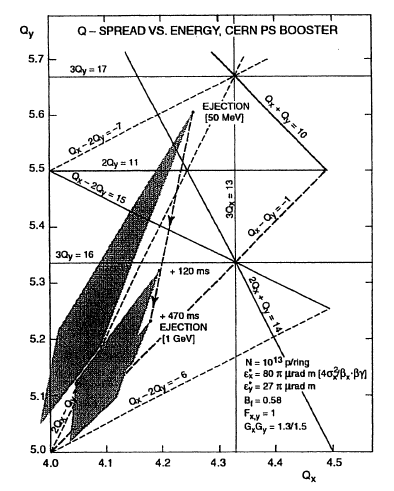
\includegraphics[width=0.7\textwidth]{Wakefields_and_Impedances/figures/tune-spread-sc.png}
\end{center}
\caption{A tune diagram illustrating the unperturbed tune of a machine, and the resulting perturbed tune and the tune spread as a result of direct space charge interactions on a bunch. Note that the tune spread has caused some particles to lie upon a major resonance harmonic. Taken from K. Schindl \cite{Schindl:SpaceCharge}.}
\label{fig:tune_diag_tune_shift}
\end{figure}

\subsubsection{Longitudinal Single Bunch Instabilities}

Similar to the change in the equations of motion for transverse particles, considering the induced fields in the longitudinal plane produces a perturbation in the longitudinal motion also. This can be thought of as an additional force alongside the electromagnetic force applied by the accelerating cavities, leading to two interesting phenomena. These are potential well distortion, occuring at bunch intensities below some stability criteria, and longitudinal mode coupling instability (LMCI) above some stability criteria.

The potential well distortion is a direct effect of the incoherent synchrotron tune shift (again, similar in nature to the tune shifts experienced in the transverse plane), which is responsible for a change in bunch length. This reveals itself from measurements by a change in the bunch length with increasing bunch intensity, as shown in Fig.~\ref{fig:pot_well_dist}. It should be noted that, depending on the source of impedance, the bunch length may increase or decrease depending on whether the bunch is above or below the transition energy of the accelerator.

\begin{figure}
\begin{center}
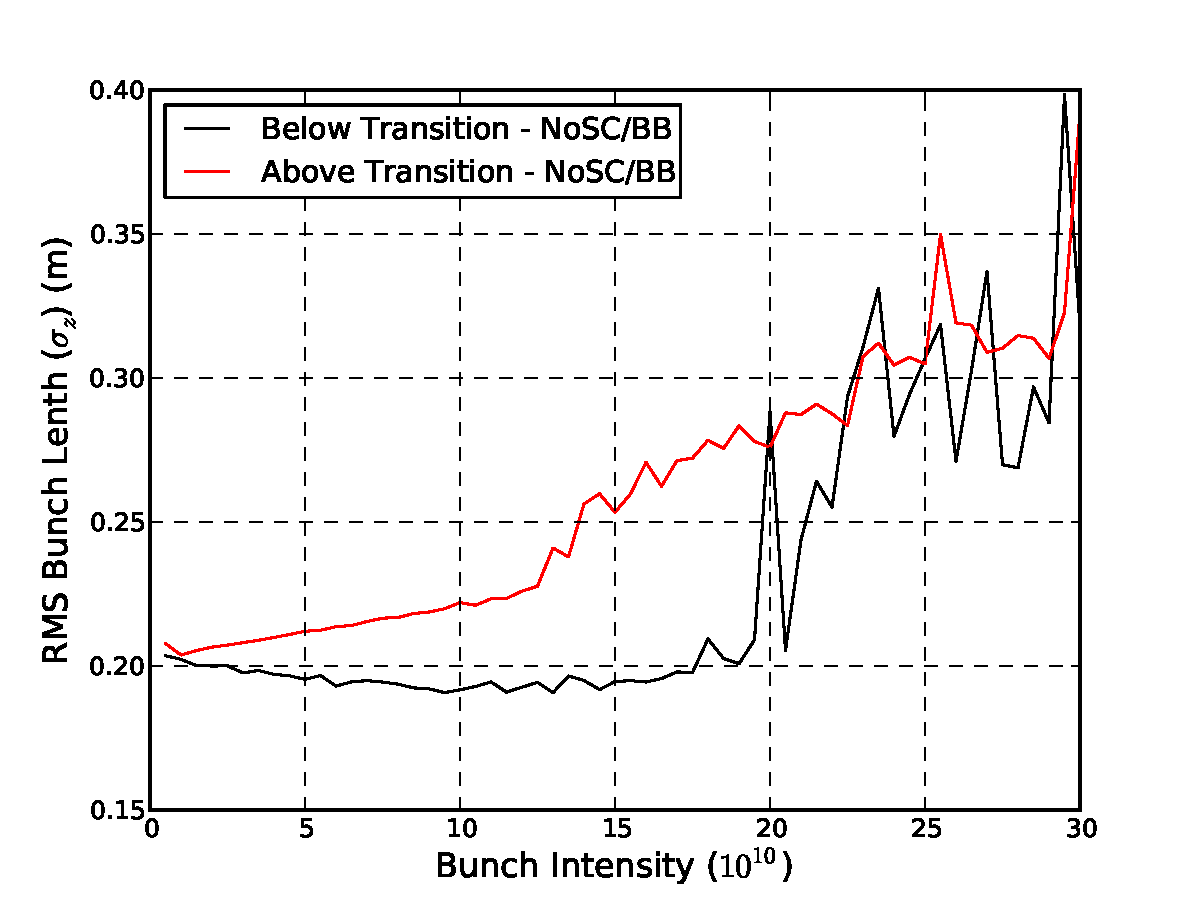
\includegraphics[width=0.7\textwidth]{Wakefields_and_Impedances/figures/rms_bunch_length_AT_BT_BB.pdf}
\end{center}
\caption{The change in the bunch length of a proton beam in the SPS due to the effects of a broadband resonator impedance ($f_{res} = 1GHz$, $R_{s}=10 \Omega$, $Q=1$) without space charge. Note that the bunch length increases when the beam is above transition, and decreases below transition, as the bunch intensity is increased.}
\label{fig:pot_well_dist}
\end{figure}

LMCI occurs when a certain intensity threshold is crossed in the accelerator, leading to a regime known as \emph{turbulent bunch lengthening}. In this mechanism the eigenfrequencies of the natural modes of oscillation of the particles within the RF bucket are shifted due to the changing potential resulting from the induced wakefield. In high intensity bunches two neighbouring modes may have their frequencies shifted to such an extent that the modes merge into one, thus leading to a case where the modes no longer have only a damped solution, but also a exponentially growing solution. This subsequently leads to the bunch oscillations becoming unstable. As can be seen in Fig.~\ref{fig:pot_well_dist}, the stable bunch intensity limit is higher below transition than above, in the case of LMCI with a broadband resonator impedance.

\subsubsection{Transverse Single Bunch Instabilities}

In the transverse plane a number of instability mechanisms apply, which can be separated into two forms, those that occur on a time scale much shorter than the synchrotron period, and those that occur on a longer time scale than the synchrotron period. In both cases the leading particles of the bunch, often called the head of the bunch, drives an oscillation in the end, or tails of the bunch. This gives these instabilities their names, the fast head-tail instability, or transverse mode coupling instability (TMCI), and the head-tail instability.

In the case of the fast head-tail instability, there are a number of transverse oscillation modes (see Fig.~\ref{fig:trans_oscillations} for examples of the transverse oscillation modes of a bunch), which as with the LMCI experience some frequency shift due to the presence of a wakefield. If the shift is large enough, two of these modes may again couple together, causing an exponential growth of the transverse size of the bunch to occur.

\begin{figure}
\begin{center}
\subfigure[]{
\label{fig:headtail-no-chrom}
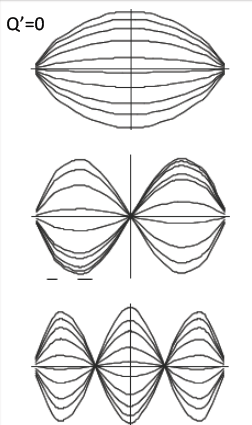
\includegraphics[width=0.3\textwidth]{Wakefields_and_Impedances/figures/headtail-no-chromaticity.png}
}
\subfigure[]{
\label{fig:headtail-with-chrom}
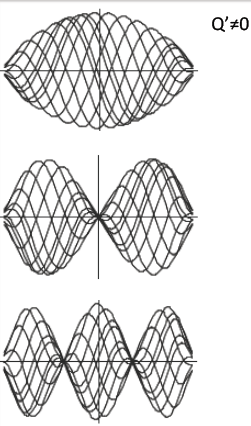
\includegraphics[width=0.3\textwidth]{Wakefields_and_Impedances/figures/headtail-with-chromaticity.png}
}
\end{center}
\caption{Examples of a number of modes of headtail oscillations without \ref{fig:headtail-no-chrom} and with \ref{fig:headtail-with-chrom} chromaticity. Note that radial and azimuthal modes may occur, as may coupled modes, in which the motion of the horizontal and vertical planes is coupled. Images courtesy of G. Rumolo \cite{Rumolo:IntroInstab}.}
\label{fig:trans_oscillations}
\end{figure}


In the case of the head-tail instability, the movement of a particle from the head of the bunch to the tail and vice versa becomes important in determining the rate of growth of any unstable modes, and whether any stabilisation mechanisms have sufficient time to damp the growth. This means that the chromaticity of the beam now takes on a great importance, as this relates the betatron tune to the longitudinal motion. This leaves the option of changing the chromaticity of the beam to act as an additional stability mechanism.

\subsubsection{Coupled Bunch Instabilities}

In addition to single bunch instabilities, it is possible in machines where multiple bunches circulate, and possessing wakefields that do not damp in the spacing between bunches (typically caused by high Q resonant impedances), that the motion of the bunch centroids themselves may become coupled together, thus driving what are called coupled bunch instabilities (TCBI for the transverse plane, LCBI for the longitudinal plane). 

This can be understood by imagining the beam as possessing M equip-spaced, equip-populated bunches. This beam will then have M possible modes of oscillation (in each case with the phase shift of $\delta \phi = 2\pi n/M$ for $n = 0,1,2..., M-1$) with a characteristic frequency of $\omega_{M}$, which may be driven by an impedance at some frequency $\omega_{0}$. If $\omega_{0} \approx n\omega_{M}$ where $n$ is an integer, then the wakefield due to the impedance may drive the oscillation either in a damped fashion (wakefield is out of phase with the oscillation of the mode) or an anti-damped fashion (wakefield is in phase with the oscillation of the mode). In the latter case, this driven oscillation may cause particle losses unless the oscillation is damped via an external mechanism, such as Landau damping \cite{Palumbo:lanDamp} or the use of a damper \cite{Schmickler:Feedback}. This motion can occur in both the longitudinal and transverse planes of motion.

